\documentclass[]{article}
\usepackage{fullpage}
\usepackage{graphicx}

\title{Chemistry Notes}
\author{Day One}
\date{Summer 2011}

\begin{document}

\maketitle

\section{Scientific notation}

Scientific notation is a way of writing numbers that makes it easy to write very large and very small numbers.

Remember that $10^{-x} = \frac{1}{10^{x}}$.

The first part of any number in scientific notation should be between one and ten in magnitude.

To convert a number to scientific notation, find the decimal point (or insert it if there isn't one), then move it so that the number is between one and ten in magnitude. Count the number of spaces you moved it; this is equal to the exponent.

\subsection{Techniques}
Count the number of places the decimal point moves to easily convert numbers to scientific notation:


\includegraphics{scientific_notation.png}

\hspace{.5cm} $5.01 \times 10^{-4}$ \hspace{4cm} $5.01 \times 10^6$

\subsection{Examples}
\begin{tabular}{ | c | c | }
    \hline
    Ordinary notation & Scientific notation \\ \hline
    50,000 & $5 \times 10^4$ \\ \hline
    50,000. & $5.0000 \times 10^4$ \\ \hline
    0.000500 & $5.00 \times 10^{-4}$ \\ \hline
\end{tabular}
\vspace{.5cm}

\section{Significant figures}

Significant figures include all digits in a number except for zeroes that act as placeholders to indicate the scale of a number. 
For multiplication and division, the result should have as many significant digits as the measured number with the smallest number of significant digits.
For addition and subtraction, the result should have as many decimal places as the measured number with the smallest number of decimal places.

\section{Dimensional analysis}

Dimensional analysis is a method of using units and conversion factors.

\subsection{Example}
The example below illustrates dimensional analysis begin used to find the number of seconds in two years.

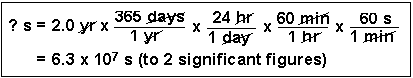
\includegraphics{dimensional_analysis.png}

\section{Prefixes}

\vspace{.5cm}
\begin{tabular}{ | c | c | c | }
    \hline
    name & symbol & magnitude \\ \hline
    tera & T & $10^{12}$ \\ \hline
    giga & G & $10^9$ \\ \hline
    mega & M & $10^6$ \\ \hline
    kilo & k & $10^3$ \\ \hline
    hecto & h & $10^2$ \\ \hline
    deca & da & $10^1$ \\ \hline
    deci & d & $10^{-1}$ \\ \hline
    centi & c & $10^{-2}$ \\ \hline
    milli & m & $10^{-3}$ \\ \hline
    micro & $\mu$ & $10^{-6}$ \\ \hline
    nano & n & $10^{-9}$ \\ \hline
    pico & p & $10^{-12}$ \\ \hline
\end{tabular}

\section{Units}

\vspace{.5cm}
\begin{tabular}{ | c | c | c | }
    \hline
    unit & symbol & type \\ \hline
    meter & m & length \\ \hline
    kilogram & kg & mass \\ \hline
    liter & L & volume \\ \hline
\end{tabular}

\section{Acknowledgements}

Some information is taken from Wikipedia, Zumdahl's \emph{Introductory Chemistry: A Foundation}, Caltech, and Texas A\&M.

\end{document}
